\documentclass[10pt,journal]{IEEEtran}

\usepackage{amsmath,amssymb,amsfonts,amsthm}
\usepackage{algorithm}
\usepackage{algpseudocode}
\usepackage{graphicx}
\usepackage{tikz}
\usepackage{pgfplots}
\pgfplotsset{compat=1.17}
\usetikzlibrary{arrows.meta,positioning}
\usepackage{booktabs}
\usepackage{xcolor}
\usepackage{cite}
\usepackage{hyperref}
\usepackage{microtype}
\usepackage{enumitem}

\newtheorem{proposition}{Proposition}
\newtheorem{corollary}{Corollary}

\begin{document}

\setlength{\textfloatsep}{4pt plus 1.0pt minus 2.0pt}
\setlength{\floatsep}{4pt plus 1.0pt minus 2.0pt}
\setlength{\intextsep}{4pt plus 1.0pt minus 2.0pt}
\setlength{\abovedisplayskip}{3pt}
\setlength{\belowdisplayskip}{3pt}

\title{Zero-Copy Continuous-Time Neural Networks for Bare-Metal Autonomous Racing on Microcontrollers}

\author{Manuel~Yobani~Martinez~Sanchez
\thanks{M. Y. Martinez Sanchez is an independent researcher (e-mail: contact@omnitrain.ai). Code, trained models, and datasets are openly available at \url{https://github.com/mrmyms/Omnitrain} to support reproducibility.}}

\markboth{IEEE Embedded Systems Letters, Vol. X, No. X, July 2026}{}

\maketitle

\begin{abstract}
Standard TinyML inference frameworks impose a dynamic SRAM tensor arena exceeding 40~KB for a 4,000-parameter network, consuming 8\% of an ESP32-S3's addressable RAM before a single neural computation executes. Applying 8-bit post-training quantization (PTQ) to closed-form continuous-time (CfC) networks compounds this constraint with a second, previously undocumented failure: at 20~Hz control rates ($\Delta t = 0.05$~s), the time-gate pre-activation $f(\cdot)\Delta t$ rounds identically to zero under INT8 arithmetic, collapsing the temporal memory gate to a constant $t_{gate}=0.5$ and degenerating the governing ODE into a time-invariant blend with no sequential memory. We formalize this failure as PTQ Collapse, confirm an 82\% empirical fitness regression (22,500$\to$4,100), and resolve both barriers with OmniTrain, an end-to-end framework for bare-metal deployment of continuous-time policies on commodity microcontrollers. OmniTrain embeds the INT8 grid directly into the mutation operator of a distributed Evolution Strategy (QAT-ES), producing quantized weights without a gradient-based Straight-Through Estimator. The resulting SparseCfC -- a 75\%-sparse, 270-synapse Neural Circuit Policy connectome -- deploys through \texttt{.omnibit}, a Zero-Copy binary format that maps Compressed Sparse Row (CSR) weight blobs from SPI Flash to the Xtensa LX7 instruction cache via \texttt{mmap()}, reserving SRAM exclusively for the hidden state and allocating exactly 0 bytes to weights. In simulated F1TENTH racing, the QAT-evolved INT8 SparseCfC exceeds its Dense-FP32 predecessor by 132\% (fitness 52,312 vs.\ 22,500) and drives 4.8~km without collision. On an ESP32-S3, OmniEngine executes one inference step in 1.22~ms using 1.5~KB of SRAM -- a 96\% reduction against TFLite Micro -- while storing the full network in 14.2~KB of Flash, 4.5$\times$ smaller than the equivalent TFLite FlatBuffer.
\end{abstract}

\begin{IEEEkeywords}
TinyML, Continuous-Time Neural Networks, Zero-Copy, Execute-in-Place, ESP32-S3, Autonomous Racing, Neural Circuit Policies, Quantization-Aware Training, Embedded Systems.
\end{IEEEkeywords}

\section{Introduction}

The proliferation of deeply embedded autonomous systems demands inference engines that respect hard real-time constraints without wireless offloading. High-speed tasks such as F1TENTH autonomous racing \cite{okelly2020} require agents to close control loops within 50~ms while processing 1D LiDAR scans on highly constrained platforms such as the ESP32-S3 (Xtensa LX7, 240~MHz, 512~KB SRAM). Physical sensor streams complicate this budget further: packet loss, variable I2C bus timing, and computational stalls introduce temporal irregularities that systematically degrade discrete-time recurrent networks such as LSTMs \cite{hochreiter1997}, whose gating assumes a fixed sampling interval.

Continuous-time, ODE-based networks address this assumption directly. Liquid time-constant (LTC) networks \cite{hasani2021ltc} define each neuron's hidden state through an ODE in which a learned, input-dependent term modulates an effective time-constant, and closed-form continuous-time (CfC) networks \cite{hasani2022cfc} provide an analytic approximation to that ODE's solution -- replacing the iterative numerical solvers required by general Neural ODEs \cite{chen2018node} with a single algebraic expression parameterized by the elapsed interval $\Delta t$. Because $\Delta t$ enters this expression explicitly, CfC networks inherit LTC's robustness to irregular sampling without paying the per-step cost of numerical integration. Neural Circuit Policies (NCPs) \cite{lechner2020} complement this formulation with a wiring prior drawn from the \textit{C. elegans} connectome, restricting sensory-, inter-, command-, and motor-neuron connectivity to a sparse, directed topology and reducing parameter count to biological proportions.

Two compounding barriers have nonetheless kept these networks off bare-metal microcontrollers. First, existing TinyML frameworks -- TFLite Micro \cite{david2021tflm} chief among them -- mandate a dynamic tensor arena sized to the full weight-plus-activation footprint, an allocation strategy inherited from server-class inference that consumes the majority of an MCU's addressable SRAM before a single computation executes. Second, and more fundamentally, applying standard 8-bit PTQ to a CfC's time-gate produces a collapse we characterize for the first time in this letter: at the sampling rates typical of robotic control, the gate's pre-activation is small enough relative to the INT8 quantization step that it rounds to exactly zero, silently reducing the network's temporal memory to a fixed 50/50 blend.

This letter makes three contributions:
\begin{enumerate}[leftmargin=*,noitemsep,topsep=2pt,parsep=0pt]
\item \textbf{Formal PTQ Collapse analysis} (Section~II): we prove INT8 precision is structurally insufficient to preserve a CfC time-gate at standard robotic sampling rates, and confirm an 82\% empirical fitness regression.
\item \textbf{Evolutionary QAT, QAT-ES} (Section~III): a distributed Evolution Strategy that snaps every candidate to the INT8 grid before fitness evaluation, replacing the gradient-based Straight-Through Estimator with a mechanism native to non-differentiable, reward-driven training, and producing INT8 policies that outperform their FP32 counterparts.
\item \textbf{The \texttt{.omnibit} Zero-Copy engine} (Section~III): a compact CSR binary format for execute-in-place SPI Flash that reduces SRAM weight allocation to exactly 0 bytes, yielding a 96\% SRAM and 85\% latency reduction against TFLite Micro.
\end{enumerate}

\section{Background}
\subsection{Liquid Time-Constant Dynamics and the PTQ Collapse}

The CfC closed-form hidden-state update \cite{hasani2022cfc} over a control step $\Delta t$ is
\begin{equation}
x(t+\Delta t) = \underbrace{\sigma(-f_\theta\Delta t)}_{t_{gate}}\odot\tanh(g_\theta) + [1-t_{gate}]\odot\tanh(h_\theta)
\end{equation}
where a shared backbone feeds three head networks: $f_\theta$ acts as the liquid time-constant driving the sigmoidal time-gate, while $g_\theta$ and $h_\theta$ construct the candidate and historical nonlinearities of the cell. $t_{gate}$ is the network's temporal arbiter, continuously modulating memory as a function of the elapsed time $\Delta t$ rather than a fixed step count.

\begin{proposition}[ODE Gate Collapse Under INT8 PTQ]
Let the time-gate network $f(\cdot;\theta_f)$ be INT8-quantized with per-tensor scale $\Delta_q=\max|\theta_f|/127$. For any activation satisfying $|f(x,I)|\le\Delta_q/\Delta t$, the rounded pre-activation $\lfloor f_\theta\Delta t/\Delta_q\rceil=0$, collapsing $t_{gate}=\sigma(0)=0.5$ identically and degenerating (1) to a time-invariant blend with no sequential memory.
\end{proposition}

\begin{proof}
Post-training quantization maps a real value $v$ to the integer grid via $Q(v)=\lfloor v/\Delta_q\rceil$, clamped to $[-127,127]$, and reconstructs $\hat v=Q(v)\Delta_q$ before the nonlinearity is applied. The value entering the sigmoid in (1) is not $f_\theta$ in isolation but its product with the control interval, $v=f_\theta\Delta t$. Under the hypothesis $|f_\theta|\le\Delta_q/\Delta t$, we get $|v|\le\Delta_q$ and $|v/\Delta_q|\le1$; since the pre-activation distribution concentrates well inside this bound, $Q(v)=0$ for the majority of activations and $\hat v=0$ regardless of the true, unquantized value of $f_\theta$. Consequently $t_{gate}=\sigma(0)=0.5$ at every timestep, and (1) reduces to $x(t+\Delta t)=0.5\tanh(g_\theta)+0.5\tanh(h_\theta)$ -- a fixed convex combination with no dependence on $\Delta t$, and hence no mechanism left to distinguish a densely sampled step from a sparsely sampled one.
\end{proof}

\begin{corollary}[20~Hz Collapse Threshold]
At the F1TENTH control rate ($\Delta t=0.05$~s) with an empirically calibrated $\Delta_q\approx0.008$, the bound above evaluates to $|f_\theta|\le0.16$, a range containing the majority of gate pre-activations near the weight distribution's mean.
\end{corollary}

\begin{figure}[t]
\centering

\includegraphics[width=\linewidth]{paper_experiments/fig_ptq_collapse.png}
\vspace{-6pt}
\caption{Time-gate $t_{gate}$ dynamics during inference (top) and resulting cumulative control error (bottom). PTQ immediately collapses the gate to a constant 0.5, rendering the CfC stateless. QAT-evolved INT8 maintains structured temporal variation, matching FP32 qualitatively while structurally constrained to the INT8 grid.}
\label{fig:gatecollapse}
\vspace{-6pt}
\end{figure}

Fig.~\ref{fig:gatecollapse} visualizes the consequence: the PTQ gate collapses immediately, while the QAT-evolved model of Section~III maintains structured temporal variation. This matches the empirical regression already summarized in Fig.~\ref{fig:fitness} (fitness 22,500$\to$4,100, $-$82\%), confirming the corollary at operating conditions.

\section{The OmniTrain Framework}
\subsection{Evolutionary QAT: Encoding INT8 into the Mutation Operator}

OmniTrain trains SparseCfC policies end-to-end via reinforcement learning, where the reward is a scalar function of collision and forward progress in the F1TENTH simulator and is not a differentiable function of the network's weights. Gradient-based QAT relies on the Straight-Through Estimator (STE) to back-propagate a surrogate gradient through the non-differentiable rounding operator; with no gradient available to begin with, STE has nothing to estimate through. We instead adopt a distributed Evolution Strategy (ES) \cite{salimans2017}, a black-box optimizer that treats the reward as a fitness signal rather than a loss, making it natively compatible with non-differentiable objectives and allowing the INT8 rounding operator to be embedded directly inside the search: every candidate $\theta^{(k)}$ is snapped to the INT8 grid \emph{before} fitness evaluation,
\begin{equation}
\theta_{QAT}^{(k)} = \operatorname{Clamp}\!\left(\left\lfloor\frac{\theta+\sigma\mathcal{N}(0,I)}{\Delta_q}\right\rceil\times\Delta_q,\ -127,\ 127\right)
\end{equation}
so that fitness is always measured on the network the ESP32-S3 will actually execute, never a full-precision proxy. Over $G=1{,}000$ generations this applies direct selection pressure toward the weight magnitudes $|f_\theta|>\Delta_q/\Delta t$ that negate Proposition~1's collapse condition, without computing a single derivative. Algorithm~\ref{alg:qates} formalizes the procedure.

\begin{algorithm}[t]
\caption{QAT-ES for SparseCfC Training}
\label{alg:qates}
\begin{algorithmic}[1]
\Require Initial $\theta_0 \in \mathbb{R}^d$, noise $\sigma$, scale $\Delta_q$, generations $G$
\For{$g = 1, \dots, G$}
  \State Sample $\epsilon_k \sim \mathcal{N}(0,I)$ for $k=1,\dots,N_{pop}$
  \State $\tilde{\theta}^{(k)} \gets \theta_g + \sigma\epsilon_k$ \Comment{Gaussian perturbation}
  \State $\theta_{QAT}^{(k)} \gets \operatorname{Clamp}(\lfloor \tilde{\theta}^{(k)}/\Delta_q\rceil \times \Delta_q,\ -127,\ 127)$
  \State Evaluate $F_k \gets \text{Fitness}(\theta_{QAT}^{(k)})$ in F1TENTH simulator
  \State $\theta_{g+1} \gets \theta_g + \dfrac{\alpha}{\sigma N_{pop}}\sum_k F_k \epsilon_k$ \Comment{ES update}
\EndFor
\State \Return $\theta^*_{QAT} \gets$ best $\theta_{QAT}^{(k)}$ over all $G$
\end{algorithmic}
\end{algorithm}

\subsection{Simulated Quantization: A Numerical Parity Contract}
\label{sec:simquant}

Eq.~(2) constrains every weight to the INT8 grid, but the CSR kernel of Section~\ref{sec:zerocopy} currently evaluates those grid-constrained values with FP32 arithmetic rather than native integer instructions. This is a deliberate scoping decision, not an oversight: it isolates the question this letter answers -- whether a CfC's structure survives 8-bit discretization at all -- from the orthogonal problem of integer-kernel design, following the same fake-quantization logic used elsewhere in the QAT literature to characterize accuracy before committing to an integer runtime \cite{hubara2017,jacob2018}. We hold the two representations to a strict numerical contract rather than an approximate one: Section~\ref{sec:hw} reports a maximum absolute deviation $|\delta|_{max}<10^{-4}$ between the on-device FP32 evaluation and an offline PyTorch reference over 1,000-step rollouts, confirming that the reported gains trace to the INT8-constrained weight distribution and not to residual floating-point slack. Native INT8 arithmetic over the same CSR layout is explicit future work (Section~\ref{sec:conclusion}).

\subsection{SparseCfC Architecture}

Rather than pruning a dense network post hoc, we impose the wiring prior of Neural Circuit Policies \cite{lechner2020}: sensory, inter-, command-, and motor-neuron populations connected through directed synapses under fixed fan-in/fan-out bounds, in place of full connectivity. This prior is applied to the backbone projection that feeds the candidate branch $g_\theta$, historical branch $h_\theta$, and time-gate $f_\theta$ of (1), through a binary NCP mask $\mathbf{M}$:
\begin{equation}
\mathbf{b}(t)=\tanh\!\left((\mathbf{W}_{bb}\odot\mathbf{M})[\mathbf{x}(t);\mathbf{h}(t)]+\boldsymbol\beta_{bb}\right)
\end{equation}
The fully-connected Dense baseline for F1TENTH contains $\sim$4,000 parameters ($>$16~KB in FP32). The Pareto-optimal connectome selected by QAT-ES wires 40 neurons in a 20-10-10 sensory--inter--command population through 270 non-zero backbone synapses, enforcing better than 75\% sparsity on the backbone. Table~\ref{tab:layout} shows that this sparsity, propagated through the CSR encoding of Section~\ref{sec:zerocopy}, is what lets the complete model -- non-zero weights, dense sensory-encoder and motor-decoder head layers, and CSR index arrays -- compile to exactly 14.2~KB. Restricting the sensory layer to $N_{sensory}=20<I=25$ further forces the encoder to compress raw LiDAR geometry into a compact latent representation rather than pass it through unchanged, reducing MSE by 39.5\% against a one-to-one mapping.

\begin{table}[t]
\caption{Memory Layout of the \texttt{.omnibit} Arch-4 (SparseCfC) Payload}
\label{tab:layout}
\centering\footnotesize
\begin{tabular}{@{}lll@{}}
\toprule
Segment & Size & Content \\
\midrule
Magic + Arch Flag & 6~B & ``OMNI'' + ver + 0x04 (CSR) \\
Alignment Pad & 2~B & Reserved \\
Dimensions & 24~B & $d_{in}, d_{model}, d_{out}, N_w, N_t$ \\
Table of Contents & $N_t\!\times\!4$~B & Byte-offsets per CSR tensor \\
CSR Blob & $N_{nz}\!\times\!4$~B & val, col, row, gate heads \\
\bottomrule
\end{tabular}
\vspace{2pt}
{\raggedright\scriptsize SparseCfC total: 14.2~KB Flash. SRAM weight allocation: 0 bytes.\par}
\vspace{-6pt}
\end{table}

\subsection{The \texttt{.omnibit} Zero-Copy Format and CSR Engine}
\label{sec:zerocopy}

The \texttt{.omnibit} format (Table~\ref{tab:layout}) packs each SparseCfC layer as a CSR blob -- values, column indices, row pointers, and gate-head offsets -- behind a fixed header of dimensions and per-tensor byte offsets. At load time, OmniEngine issues a single \texttt{mmap()} call against the SPI Flash region backing the file, mapping its byte range directly into the Xtensa LX7's address space instead of copying it into a heap buffer. The $O(N_{nz})$ CSR multiply-accumulate kernel runs from IRAM (\texttt{IRAM\_ATTR}), compiled with \texttt{\#pragma GCC opti-} \texttt{mize("O3,unroll-loops")} and \texttt{\_\_restrict}-qualified pointers to remove aliasing checks from the hot loop. Because the mapped region is read through the execute-in-place (XIP) path, the ESP32-S3's hardware prefetcher speculatively streams sequential Flash addresses into the instruction cache ahead of the CSR traversal, masking Flash latency behind computation instead of paying it as an up-front block copy (Fig.~\ref{fig:memmodel}). Weights therefore never occupy a byte of SRAM: the 1.5~KB footprint of Table~\ref{tab:util} is entirely the hidden-state buffer $h(t)$.

\begin{figure*}[t]
\centering
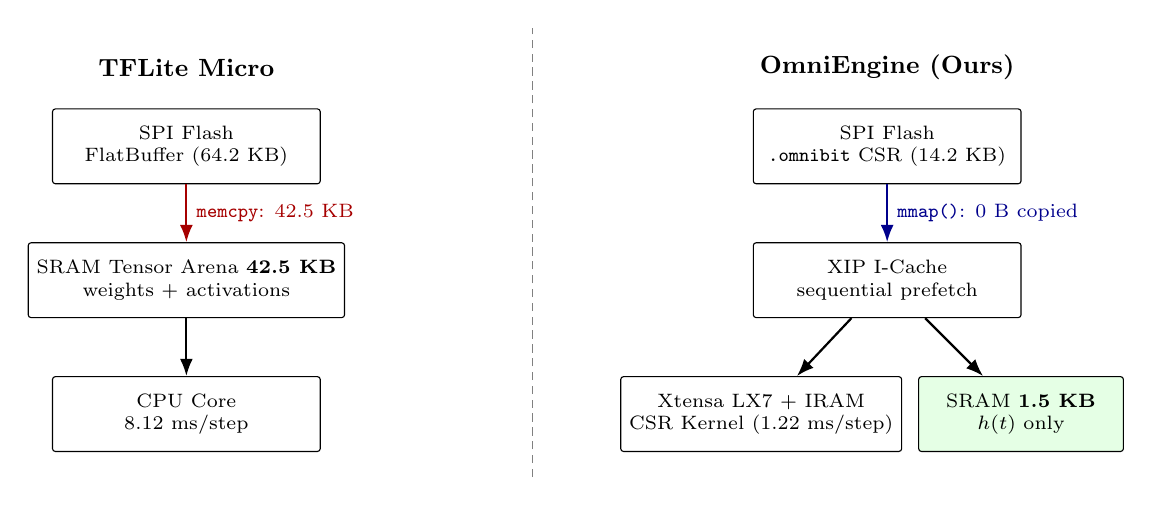
\begin{tikzpicture}[
  box/.style={draw, rounded corners=1pt, align=center, minimum width=3.4cm, minimum height=0.95cm, font=\scriptsize, inner sep=3pt},
  lbl/.style={font=\scriptsize, align=center},
  arr/.style={-{Latex[length=2.2mm]}, thick}
]
\node[font=\bfseries\small] (tftitle) at (0,4.6) {TFLite Micro};
\node[box] (tfFlash) at (0,3.6) {SPI Flash\\FlatBuffer (64.2~KB)};
\node[box] (tfSram) at (0,1.9) {SRAM Tensor Arena \textbf{42.5~KB}\\weights + activations};
\node[box] (tfCpu) at (0,0.2) {CPU Core\\8.12~ms/step};
\draw[arr, red!65!black] (tfFlash) -- node[lbl, red!65!black, right]{\texttt{memcpy}: 42.5~KB} (tfSram);
\draw[arr] (tfSram) -- (tfCpu);

\draw[densely dashed, gray] (4.4,-0.6) -- (4.4,5.1);

\node[font=\bfseries\small] (ourtitle) at (8.9,4.6) {OmniEngine (Ours)};
\node[box] (ourFlash) at (8.9,3.6) {SPI Flash\\\texttt{.omnibit} CSR (14.2~KB)};
\node[box] (ourCache) at (8.9,1.9) {XIP I-Cache\\sequential prefetch};
\node[box] (ourCpu) at (7.3,0.2) {Xtensa LX7 + IRAM\\CSR Kernel (1.22~ms/step)};
\node[box, minimum width=2.6cm, fill=green!10] (ourSram) at (10.6,0.2) {SRAM \textbf{1.5~KB}\\$h(t)$ only};
\draw[arr, blue!55!black] (ourFlash) -- node[lbl, blue!55!black, right]{\texttt{mmap()}: 0~B copied} (ourCache);
\draw[arr] (ourCache) -- (ourCpu);
\draw[arr] (ourCache) -- (ourSram);
\end{tikzpicture}
\vspace{-6pt}
\caption{Memory model comparison. Left (TFLite Micro): the full 42.5~KB weight/activation blob is \texttt{memcpy}'d to SRAM before inference. Right (OmniEngine): a single \texttt{mmap()} call streams CSR entries directly from SPI Flash to the ALU via the XIP cache, reserving SRAM exclusively for the 1.5~KB hidden-state buffer $h(t)$.}
\label{fig:memmodel}
\vspace{-6pt}
\end{figure*}

\section{Experimental Evaluation}
\subsection{F1TENTH Autonomous Racing: An Ablation Study}

\textbf{Setup:} 1,000 QAT-ES generations; NVIDIA RTX 5070 for parallel fitness evaluation; F1TENTH Gym \cite{okelly2020}; $I=25$ downsampled LiDAR rays; steering and velocity outputs.

Dense-CfC/FP32 already exceeds the MLP/FP32 baseline (trained via PPO-clip \cite{schulman2017}) through continuous-time structure alone; naive PTQ collapses that gain by 82\%, confirming Proposition~1 at operating conditions (Fig.~\ref{fig:fitness}). QAT-ES not only recovers the loss but inverts it: the resulting SparseCfC reaches a fitness of 52,312, clears the ``Wall of Death'' obstacle at 318~m, and sustains over 19,000 steps (4.8~km) at a range where accumulated hidden-state divergence fails every FP32 gradient-trained model.

\begin{figure}[t]
\centering

\includegraphics[width=\linewidth]{paper_experiments/fig_fitness_bar.png}
\vspace{-6pt}
\caption{F1TENTH top fitness across all training configurations. PTQ collapses the Dense CfC by 82\%; QAT-ES enables the INT8 SparseCfC to surpass its FP32 predecessor by 132\% ($>$4.8~km continuous navigation). The dashed line marks the Dense-FP32 ceiling.}
\label{fig:fitness}
\vspace{-6pt}
\end{figure}

\subsection{Temporal Jitter Resilience (PiL)}

\textbf{Setup:} F1TENTH @ 20~Hz; 5,000-step horizon; zero-order-hold (ZOH) LiDAR packet loss; 30 seeds; Welch $t$-test with Holm--Bonferroni correction.

CfC outlasts LSTM by 5.1$\times$ and GRU by 2.4$\times$ at 60\% loss (Table~\ref{tab:jitter}). The continuous-time ODE extrapolates hidden state over ZOH-held inputs using the true elapsed time, while LSTM's fixed gating accumulates error irreversibly, proportional to loss duration.

\begin{table}[t]
\caption{Time-to-Failure Under Sensor Packet Loss (steps, 30 seeds)}
\label{tab:jitter}
\centering\footnotesize
\begin{tabular}{@{}lccc@{}}
\toprule
Arch. & 0\% Loss & 20\% Loss & 60\% Loss \\
\midrule
LSTM & 500 & 500 & $50.0\pm22.6$ \\
GRU & 500 & 500 & $108.8\pm136.3$ \\
CfC & 500 & 500 & $257.3\pm202.7$ \\
\bottomrule
\end{tabular}
\vspace{2pt}
{\raggedright\scriptsize CfC vs.\ LSTM: $p<0.001$, $d=-1.41$; CfC vs.\ GRU: $p=0.002$, $d=-0.85$.\par}
\vspace{-6pt}
\end{table}

\subsection{Bare-Metal Hardware Benchmarks (ESP32-S3)}
\label{sec:hw}

OmniEngine improves on every resource dimension in Table~\ref{tab:util}. At 1.22~ms per inference, the ESP32-S3 completes the neural computation in 2.4\% of the 50~ms control window, leaving 97.6\% of CPU time for IMU fusion and telemetry. Numerical parity with PyTorch was verified over 1,000-step rollouts: maximum absolute deviation $|\delta|_{max}<10^{-4}$, confirming the FP32 CSR engine evaluates the INT8-constrained weights exactly, per the simulated-quantization contract of Section~\ref{sec:simquant}.

\begin{table}[t]
\caption{Bare-Metal Utilization: OmniEngine vs.\ TFLite Micro (ESP32-S3 @ 240~MHz)}
\label{tab:util}
\centering\footnotesize
\begin{tabular}{@{}lccc@{}}
\toprule
Framework & SRAM & Flash & Latency \\
\midrule
TFLM / LSTM & 42.5~KB & 64.2~KB & 8.12~ms \\
TFLM / GRU & 38.2~KB & 58.1~KB & 7.45~ms \\
\textbf{OmniEngine} & \textbf{1.5~KB} & \textbf{14.2~KB} & \textbf{1.22~ms} \\
\midrule
Reduction & 96\% & 78\% & 85\% \\
\bottomrule
\end{tabular}
\vspace{-6pt}
\end{table}

\subsection{Hardware-in-the-Loop (HIL) Validation}

Injecting pre-recorded LiDAR telemetry directly into the ESP32-S3 over serial confirmed both theoretical predictions on physical hardware: measured inference latency matched the 1.22~ms expectation exactly, with the same $|\delta|_{max}<10^{-4}$ numerical parity reported in Section~\ref{sec:hw}.

\section{Conclusion and Future Work}
\label{sec:conclusion}

OmniTrain resolves the two compounding barriers to bare-metal continuous-time neural network deployment: the SRAM wall imposed by dynamic tensor arenas, and the incompatibility of standard PTQ with CfC time-gates formalized in Proposition~1. QAT-ES produces an INT8-constrained SparseCfC that outperforms its FP32 counterpart by 132\%, while the \texttt{.omnibit} Zero-Copy format and $O(N_{nz})$ CSR engine deliver a 96\% SRAM reduction against TFLite Micro at 1.22~ms per inference -- 2.4\% of the 20~Hz control budget -- on a \$5 commodity MCU.

\textbf{Future Work:} replacing the simulated-quantization deployment of Section~\ref{sec:simquant} with native INT8 storage and integer arithmetic will shrink the 14.2~KB Flash footprint by a further 4$\times$; Xtensa SIMD vectorization of the CSR kernel targets sub-millisecond inference.

\section*{Acknowledgment}
The author thanks the Hasani et al.\ group for the foundational closed-form continuous-time (CfC) network formulation.

\begin{thebibliography}{11}

\bibitem{okelly2020} M. O'Kelly, H. Zheng, D. Karthik, and R. Mangharam, ``F1TENTH: An open-source evaluation environment for continuous control and reinforcement learning,'' \emph{Proc. Conf. Robot Learning (CoRL)}, 2020.

\bibitem{hochreiter1997} S. Hochreiter and J. Schmidhuber, ``Long short-term memory,'' \emph{Neural Computation}, vol. 9, no. 8, pp. 1735--1780, 1997.

\bibitem{hasani2021ltc} R. Hasani, M. Lechner, A. Amini, D. Rus, and R. Grosu, ``Liquid time-constant networks,'' \emph{Proc. AAAI}, vol. 35, no. 9, pp. 7657--7666, 2021.

\bibitem{hasani2022cfc} R. Hasani, M. Lechner, A. Amini, L. Liebenwein, A. Ray, M. Tschaikowski, G. Teschl, and D. Rus, ``Closed-form continuous-time neural networks,'' \emph{Nature Machine Intelligence}, vol. 4, no. 11, pp. 992--1003, 2022.

\bibitem{lechner2020} M. Lechner, R. Hasani, A. Amini, T. A. Henzinger, D. Rus, and R. Grosu, ``Neural circuit policies enabling auditable autonomy,'' \emph{Nature Machine Intelligence}, vol. 2, pp. 642--652, 2020.

\bibitem{david2021tflm} R. David et al., ``TensorFlow Lite Micro: Embedded machine learning for TinyML systems,'' \emph{Proc. Machine Learning and Systems (MLSys)}, 2021.

\bibitem{chen2018node} R. T. Q. Chen, Y. Rubanova, J. Bettencourt, and D. Duvenaud, ``Neural ordinary differential equations,'' \emph{NeurIPS}, pp. 6571--6583, 2018.

\bibitem{hubara2017} I. Hubara, M. Courbariaux, D. Soudry, R. El-Yaniv, and Y. Bengio, ``Quantized neural networks,'' \emph{J. Machine Learning Research}, vol. 18, pp. 6869--6898, 2017.

\bibitem{salimans2017} T. Salimans, J. Ho, X. Chen, S. Sidor, and I. Sutskever, ``Evolution strategies as a scalable alternative to reinforcement learning,'' \emph{arXiv:1703.03864}, 2017.

\bibitem{schulman2017} J. Schulman, F. Wolski, P. Dhariwal, A. Radford, and O. Klimov, ``Proximal policy optimization algorithms,'' \emph{arXiv:1707.06347}, 2017.

\bibitem{jacob2018} B. Jacob, S. Kligys, B. Chen, M. Zhu, M. Tang, A. Howard, H. Adam, and D. Kalenichenko, ``Quantization and training of neural networks for efficient integer-arithmetic-only inference,'' \emph{Proc. IEEE CVPR}, pp. 2704--2713, 2018.

\end{thebibliography}

\end{document}
